\documentclass[10pt,twoside]{article}

\usepackage[english]{babel}
\usepackage[OT1]{fontenc}
\usepackage[utf8]{inputenc}
\usepackage{graphicx}
\usepackage{url}
\usepackage{hyperref}
\usepackage{cite}
\usepackage{fancyhdr}
\usepackage[margin=1.3in]{geometry} % Set custom page margins

\pagestyle{fancy} % Set the page style to fancy
\fancyhf{}
\fancyhead{} % Clear the header
\fancyfoot[C]{\thepage} % Center the page number at the bottom

\renewcommand{\headrulewidth}{0pt} % Remove header line

\title{Protection of Private Data Against Web Scraping}

\author{Jakub Ján Zuber\\[2pt]
  {\small Slovak University of Technology in Bratislava}\\
  {\small Faculty of Informatics and Information Technologies}\\
  {\small \texttt{xzuber@stuba.sk}}
}

\date{\small 5th November 2023}

\begin{document}

\maketitle
\newpage

\begin{abstract}
My work is going to be mainly focused on the protection of important people within companies against this technique. People employed at positions of CEO, CFO, COO are often targets of whaling by hacking/scamming groups. This is caused by their huge influence and access to bank accounts of their big companies. Due to the number of interviews and public information available, it is hard for them to keep their lives private. After introducing the problems, I will introduce a couple of already existing solutions and try to design algorithms capable of detecting web scraping tools/bots. Together with that, I will evaluate some of the training methods that are used to teach privacy protection to this group of people. In my work, I plan on including interviews with people in leading positions as well. Their answers will be evaluated in conjunction with training methods.
\end{abstract}
\newpage

\section{Introduction}
% Your introduction content goes here.
% * What is webscraping, why is it, how does it work
% ! general information
In the past few years, the number of scamming attempts increased.  One of the most common methods of gaining data for this type of attack is web scraping. As defined by (cite wiki )Wikipedia web scraping is characterised as `Web scraping, web harvesting, or web data extraction is data scraping used for extracting data from websites`.

In a less specific way, web scraping can be characterised as any activity either by humans or robots whose purpose is to download data from the website, structure it and save it in file format such as spreadsheet, JSON or other. The legality of this activity is questionable from any point of view. Depending on the actor, data extracted and purpose, we can try to decide on the definitive answer for each case. (cite A Dive into Web Scraper World). The groundwork for this type of lawsuit was set in the early 2000s by companies such as eBay or Facebook. However, big companies are not the only ones being hit by web scraping tools. CEOs, CFOs and other corporate employees in top-tier positions face the same issues. Many entities try every day to steal their identities and find out about their privacy as much as possible. This information can be later used in further hacking attempts. 

How to combat web scrapers? I am going to explain some of the most common methods and dive into the algorithms used in these operations. In the end, I will include real-world experiences from people exposed to this problem.

\section{Role of web scraping in data collection}\label{data-privacy}
% * What is data privacy, how to protect against it, what are most commong problems
As stated in web article What Is Data Collection: Methods, Types, Tools \cite{simplilearn-data-collection} data collection as concept is with is for centuries. Few things that changed are method. These changed quite a bit. Development of methods is a natural process that always occured. One thing that has changed drastically is size of datasets. In the past, when somebody was trying to gain information it was hard and mostly done by talking to people or researching books. These days number of sources is much bigger and they are much more widespread between people. This was allowed by inventions such as WorldWideWeb. In it's core, WorldWideWab is just a database of various information from many different sources.
According to already mentioned article \cite{simplilearn-data-collection} we divide resources into two general categories

\begin{enumerate}
  \item Primary resources
    \begin{enumerate}
      \renewcommand{\theenumi}{\alph{enumi}} % Change the inner list numbering to lowercase letters
      \item Surveys and Questionnaires
      \item Interviews
      \item Observations
      \item Experiments
      \item Focus groups
    \end{enumerate}
  \item Secondary resources
    \begin{enumerate}
      \renewcommand{\theenumi}{\alph{enumi}} % Change the inner list numbering to lowercase letters
      \item Published Sources
      \item Online Databases
      \item Government and Institutional records
      \item Publicly available data
      \item Past research studies
    \end{enumerate}
\end{enumerate}
The main data collection category that i am going to focus on is Publicly available data and Online databases. Publicky available data is every resource from book, news article all the way to data stored on the internet. Due to this reason, these two categories are connected together. The online database is separate category due to the fact that it may not always be publicly available resource. Databases may sometimes be protected from public access. This does not always stop web-scraping bots from accessing this data. This action is not so common due to its legal reprocutions as this is considered illegal access to private data (hacking).

While the web scraping is now always the number one choice of gaining knowledge of somone's private data it plays important middle step between knowning the subject and having no idea about him/her at all.

Some of the problems related to web scraping are CAPTCHAs, page structure changes or dynamic content. Due to the nature of HTML websites they are unstructured which causes problems for web scrapers which try to operate and save data in structured ways. Second problem related to this area is that various websites have different structures, different designs and use multiple technologies such as JS, Django, XML, CSS ... . 
\subsection{Data technologies}

\subsection{Legality}

\section{Web scraping methods and approaches}\label{methods-approaches}

\begin{figure}[htp]
  \centering
  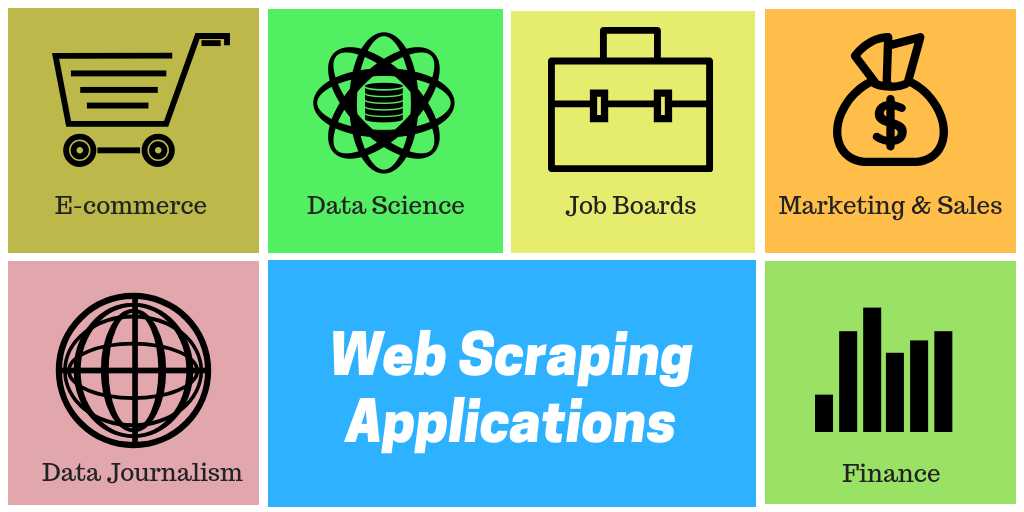
\includegraphics[width=0.5\textwidth]{photo1}
  \caption{Applications of web scraping\cite{towardsdatascience-web-scraping}}
  
\end{figure}
% Content of this section.

\section{Retrieval systems}\label{even-more-important-section}
% Content of this section.

\section{Protection algorithms}\label{protection-algorithms}
\subsection{Scrapy}
\subsection{Coding}
% Content of this section.

\section{Real life experience}\label{real-life-experience}
In my short IT experience I had luck to be by side of my manager when solving scamming issue at my workplace. Because of this I learned power of webscraping in retrieval of private data. In this particular scam, scammer used publicly available information of CFO at this company. The scammer used web articles in which he was interviewed about his past and current employments. This scam was luckily not succesfull yet it thought me a lot about this world. It was perfect case study of well planned scam which utilised multiple technologies, resources and methods. Web scraping was one of them. Because of this, I decide to interview my manager and CFO for this article.
% Content of this section.
% ! include questionare

\subsection{Some Explanation}\label{explanation}
% Content of this subsection.

\subsection{More Explanation}\label{more-explanation}
% Content of this subsection.

\section{Conclusion}\label{conclusion}
% Your conclusion content goes here.

\newpage
% Generate the bibliography from the 'references.bib' file
\bibliography{references}
\bibliographystyle{abbrv} % Choose your preferred bibliography style.

\cite{wikiscraping}
\cite{dive-into-web-scraping}
\cite{simplilearn-data-collection}
\cite{towardsdatascience-web-scraping}

\end{document}
